\chapter{Grundlagen}

% erster schritt ein datensatz suchen!!!!! nachlesen in visualisation buch

% 1. Datenquellen @ p 26

% definieren daten und so. lesen visualisation.

% 2. erwähnen: abhängige und unabhängige variable. verschieden, wenn verschiedene dimensionen.

\section{2-Dimensionales Punktediagramm}

% now the cool part comes

Das 2-Dimensionale Punktediagramm ist der am meisten verwendete Typ des Punktediagramms. Sie nutzen die sehr guten Fähigkeiten des Menschen aus, relative Positionen einzuschätzen und vergleichen zu können \cite{viz}.

Bei unserem 

%sagen dass 2d am meisten verwendet ist

%skalen (range x und y, skalierung(lineare skalierung, oft gebraucht))


\subsection{Interpolation}

% das gleiche erzählen wie vorher zitieren usw

Für eine verbesserte Ansicht des Punktediagramms fügt man oft eine Linie ein, die alle im Punktediagramm vorhandenen Punkte verbindet. Sie stellt den Verlauf des Wertes zwischen den Datenpunkten dar.

Die unkomplizierteste, am meisten Verwendete Interpolation ist die \textbf{lineare Interpolation} (Abbildung \ref{fig:linear}). Zwei nebeneinanderliegende Punkte werden durch einer Gerade verbunden.

\begin{figure}[htbp]
	\centering
	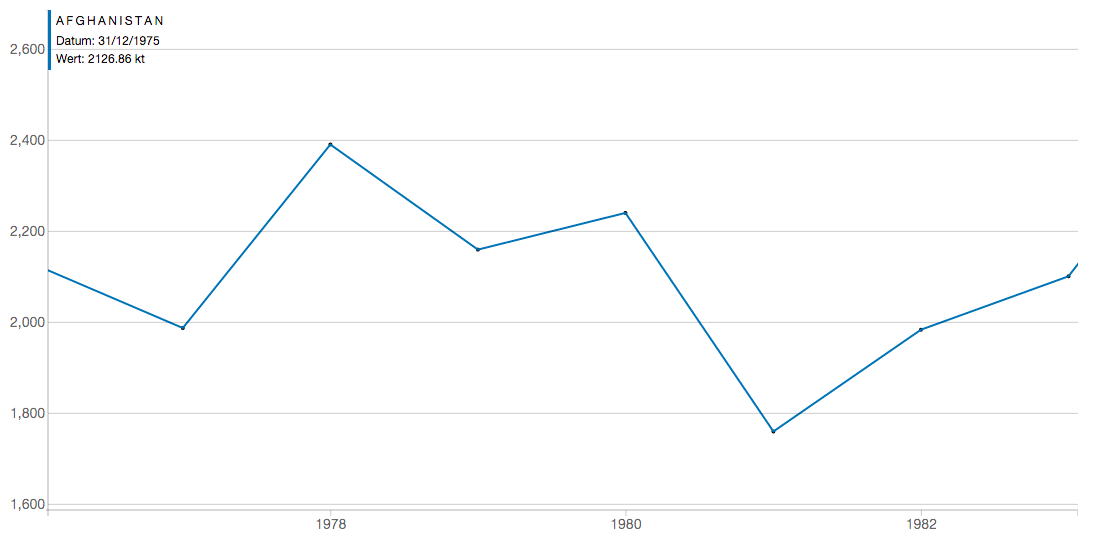
\includegraphics[width=0.80\linewidth]{images/linear}
	\caption[Lineare Interpolation]{Beispiel der linearen Interpolation am Datensatz des CO2-Verbrauchs von Afghanistan. <zu test layout verlinken>}
	\label{fig:linear}
\end{figure}

Die Interpolation mit Splines, der \textbf{Kubisch Hermitescher Spline} (Abbildung \ref{fig:cardinal}).

\begin{figure}[htbp]
	\centering
	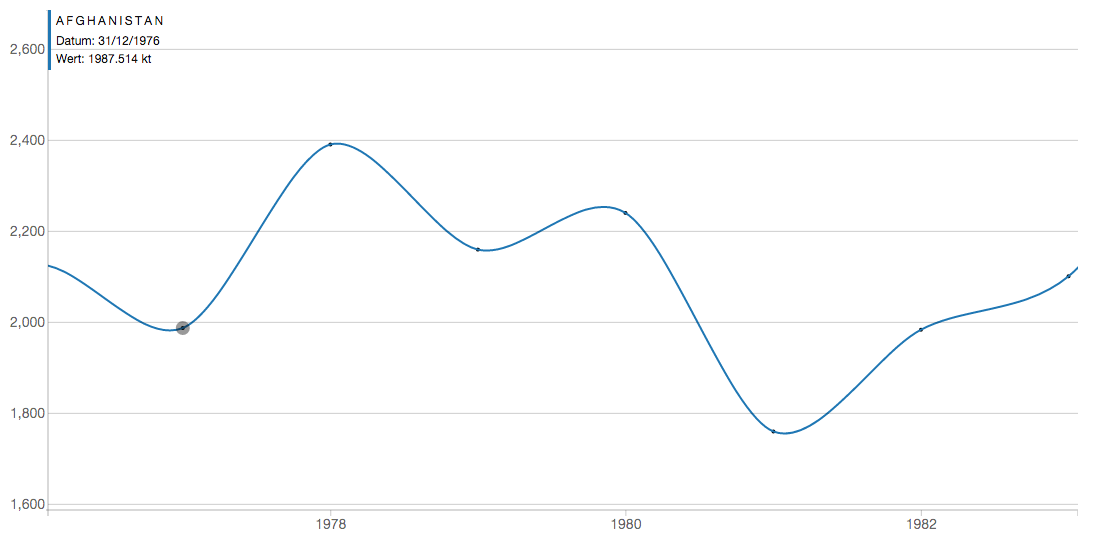
\includegraphics[width=0.80\linewidth]{images/cardinal}
	\caption[Kubischer Hermitescher Spline]{Beispiel des Kubischen Hermetischen Spline am Datensatz des CO2-Verbrauchs von Afghanistan <zu test layout verlinken>}
	\label{fig:cardinal}
\end{figure}

\subsection{Linien}
\subsection{Tooltip}
\subsection{Anzeige von mehreren Datensätzen}

\section{3-Dimensionaler Punktediagramm}

\subsection{Kamera}
\subsection{Projektion}
\subsection{Orthogonale und Perspektivische Projektion}
\subsection{Transition zwischen Projektionen}

\section{n-Dimensionaler Punktediagramm}